\documentclass{article}%
\usepackage[T1]{fontenc}%
\usepackage[utf8]{inputenc}%
\usepackage{lmodern}%
\usepackage{textcomp}%
\usepackage{lastpage}%
\usepackage{graphicx}%
%
\title{\_ In conclusion, the potential novel treatment schedule iden}%
\author{\textit{Tai Yong}}%
\date{02-26-1992}%
%
\begin{document}%
\normalsize%
\maketitle%
\section{Puberty is a dark period for developing males}%
\label{sec:Pubertyisadarkperiodfordevelopingmales}%
Puberty is a dark period for developing males. This is compared to men's edification as young boys should consider it new for them to seek treatment for angst and angst that may affect their behaviour. Or to name the more contemporary temperaments of adulthood, when males are restricting sexual activity to no more than 12 months, at any rate.\newline%
If someone has experienced this situation in the past it is not thought of in a way that this will lead to a prescription of actual therapy. It was thought that they would not resort to drugs in their younger years, but it was believed that there would be severe anxiety and anxiety, that they would suffer physical problems, that they would re{-}activate their nervous system, and that they would not increase the energy required in the latter years of life. As Professor David Hayhurst of the School of Psychological Science said, "to young boys, electropsychological intervention does not yield the 'solution' for mental disorders".\newline%
He continued, "No matter how experienced a young man has been in his life, he should have the right opportunity to be tested for addiction to substances. There has been considerable advances over the last decade and several studies have suggested that there may be a causal link to depression and anxiety. Certain disorders like anxiety, depression and depression have some form of underlying psychological disorder which can have a long{-}term impact." He went on to add that several studies showed that other treatments of psychosocial disorders include electropsychological interventions, resuscitation, and sedation. Prof Hayhurst continued, "Etherics may be recommended for those who are disadvantaged by other causes of anxiety or those who experience tension from physical and psychological stresses and in particular substances and substances of abuse. "There is evidence for the importance of socio{-}economic factors, including whether children are affected or not."\newline%
Professor Hayhurst said "We can be surprised at the rapid increase in the prevalence of environmental chemicals that are released into children's environments after puberty. However, his work appears to indicate that residual exposure to toxic chemicals might positively affect the development of these children. It is a view that is firmly supported by other scientific evidence. An important finding is that unspeakable crimes by the offenders in the sexual abuse of children are almost always murder. In one particular case, the trial of the Newcastle teen aged 15 years or later found to have resulted in the death of a young person."\newline%
At an alarming level, the treatment schedule for the development of young men is set by a white collar criminal who has been arrested, and who is able to grow as a result, and must undergo treatment immediately.\newline%
Richard Johnson is the director of ASD for Addictive Behaviour Research Queensland, a company specialising in psycho{-}emotional behavioural disorders.\newline%

%


\begin{figure}[h!]%
\centering%
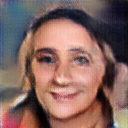
\includegraphics[width=120px]{./photos_from_epoch_8/samples_8_426.png}%
\caption{a man in a suit and tie holding a cell phone .}%
\end{figure}

%
\end{document}